\documentclass[10pt,a4paper]{article}
\usepackage[margin=1.8cm]{geometry}
\usepackage{booktabs}
\usepackage{array}
\usepackage{xcolor}
\usepackage{colortbl}
\usepackage{caption}
\usepackage{enumitem}
\usepackage{titlesec}
\usepackage{tabularx}
\usepackage{amsmath}
\usepackage{amssymb}
\usepackage{multirow}
\usepackage{pgfplots}
\pgfplotsset{compat=1.17}
\usepackage{tikz}

\titlespacing*{\section}{0pt}{8pt}{3pt}
\titlespacing*{\subsection}{0pt}{6pt}{2pt}
\setlength{\parskip}{2pt}
\setlength{\parindent}{0pt}

\definecolor{bestrow}{RGB}{215,240,215}
\definecolor{badrow}{RGB}{250,225,225}
\definecolor{barblue}{RGB}{60,120,200}
\definecolor{bargold}{RGB}{220,165,40}

\begin{document}

\begin{center}
{\Large\bfseries PS-SSR: Methods Beating Pure SSR on 6Q Benchmark}\\[3pt]
{\small Qwen3-8B (bf16) $\cdot$ 66 clusters $\cdot$ $\sim$12K posts $\cdot$ 6 original survey questions $\cdot$ Mean Jensen-Shannon divergence}\\[2pt]
{\footnotesize Baseline: Direct SSR $=$ \textbf{0.0277}. Lead method: \textbf{SSR + LLM-dist (w=0.5) $=$ 0.0257}, $-$7.2\%.}
\end{center}

\vspace{-4pt}\hrule\vspace{6pt}

\section*{1. Methods}

\newcommand{\mheader}[2]{\textbf{#1} --- #2}

\mheader{M0 Pure SSR (baseline)}{Embedding-based. Embed cluster posts and the 5 anchor options; per-cluster distribution is softmax of anchor-to-post similarity. Aggregate uniformly over top-$K$ clusters. No LLM at inference.}

\mheader{M1 LLM-dist}{For each cluster, feed the LLM a sample of posts and the 5 anchors in a single prompt; the LLM outputs a probability over the anchors directly (not per-post voting). Aggregate across clusters.}

\mheader{M2 SSR + LLM-dist ensemble $\bigstar$}{Linear mix of M0 and M1: $P = w \cdot P_{\text{SSR}} + (1-w) \cdot P_{\text{LLM-dist}}$. Best at $w=0.5$.}

\mheader{M3 Multi-layer persona-steered generation}{Extract a per-cluster persona direction from mean hidden states at layers $\{16, 20, 24\}$. At generation, add all three steering vectors simultaneously, sample $n$ responses per cluster, then run SSR on the steered outputs.}

\mheader{M4 SSR + ML-steer ensemble}{Linear mix of M0 and M3: $P = w \cdot P_{\text{SSR}} + (1-w) \cdot P_{\text{ML-steer}}$. Best at $w = 0.5$--$0.7$.}

\mheader{M5 SSR knob tuning}{Pure SSR with swept posts-per-cluster $n$ or top-$K$. No LLM.}

\vspace{6pt}\hrule\vspace{6pt}

\section*{2. Master Leaderboard}

\begin{minipage}[t]{0.57\textwidth}
\captionof{table}{Mean JS on 6Q ($\downarrow$ better)}
\centering\small
\begin{tabular}{@{}rlcc@{}}
\toprule
\# & Method & Mean JS & $\Delta$ vs M0 \\
\midrule
\rowcolor{bestrow} 1 & M2: SSR + LLM-dist, $w$=0.5 & \textbf{0.0257} & \textbf{$-$7.2\%} \\
2 & M2: SSR + LLM-dist, $w$=0.6 & 0.0258 & $-$6.9\% \\
3 & M2: SSR + LLM-dist, $w$=0.7 & 0.0259 & $-$6.5\% \\
4 & M1: LLM-dist top-10       & 0.0259 & $-$6.5\% \\
5 & M2: SSR + LLM-dist, $w$=0.8 & 0.0261 & $-$5.8\% \\
6 & M4: SSR + ML-steer, $w$=0.5 & 0.0261 & $-$5.4\% \\
7 & M4: SSR + ML-steer, $w$=0.7 & 0.0264 & $-$4.3\% \\
8 & M4: SSR + ML-steer, $w$=0.9 & 0.0267 & $-$3.3\% \\
9 & M5: SSR top-5 clusters    & 0.0272 & $-$1.8\% \\
10 & M5: SSR $n$=50 posts     & 0.0275 & $-$0.7\% \\
\midrule
--- & \textit{M0: Pure SSR baseline} & \textit{0.0277} & --- \\
\bottomrule
\end{tabular}
\end{minipage}
\hfill
\begin{minipage}[t]{0.40\textwidth}
\vspace{14pt}
\captionof{figure}{Mean JS (shorter $=$ better)}
\centering
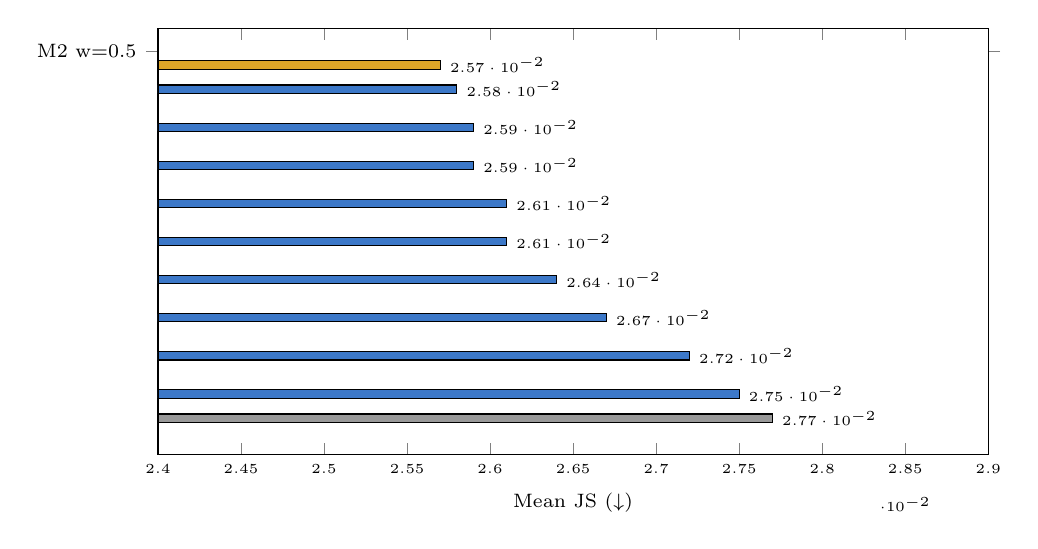
\begin{tikzpicture}
\begin{axis}[
  xbar, bar width=3pt, width=\linewidth, height=7cm,
  xmin=0.024, xmax=0.029,
  xlabel={Mean JS ($\downarrow$)}, xlabel style={font=\scriptsize},
  ytick=data, yticklabel style={font=\scriptsize, align=right},
  xticklabel style={font=\tiny},
  symbolic y coords={
    M2 w=0.5,M2 w=0.6,M2 w=0.7,M1 top-10,
    M2 w=0.8,M4 w=0.5,M4 w=0.7,M4 w=0.9,
    M5 top-5,M5 n=50,M0 SSR},
  nodes near coords, nodes near coords style={font=\tiny},
  y dir=reverse,
  enlarge y limits=0.06,
]
\addplot[fill=bargold] coordinates {(0.0257,M2 w=0.5)};
\addplot[fill=barblue] coordinates {
  (0.0258,M2 w=0.6) (0.0259,M2 w=0.7) (0.0259,M1 top-10)
  (0.0261,M2 w=0.8) (0.0261,M4 w=0.5) (0.0264,M4 w=0.7)
  (0.0267,M4 w=0.9) (0.0272,M5 top-5) (0.0275,M5 n=50)};
\addplot[fill=black!40] coordinates {(0.0277,M0 SSR)};
\end{axis}
\end{tikzpicture}
\end{minipage}

\vspace{8pt}
\section*{3. Per-question JS (top methods)}

\centering
\small
\begin{tabular}{@{}lcccccc@{}}
\toprule
Method & Q1 \texttt{8.0/3} & Q2 \texttt{8.0/4} & Q3 \texttt{9.0/3} & Q4 \texttt{9.0/4} & Q5 \texttt{9.0/5} & Q6 \texttt{11.0/3} \\
\midrule
\rowcolor{bestrow} M2 SSR+LLMdist $w$=0.5 & 0.0098 & 0.0483 & 0.0330 & 0.0155 & 0.0339 & 0.0139 \\
M2 SSR+LLMdist $w$=0.6 & 0.0103 & 0.0476 & 0.0303 & 0.0157 & 0.0362 & 0.0146 \\
M2 SSR+LLMdist $w$=0.7 & 0.0109 & 0.0470 & 0.0275 & 0.0159 & 0.0386 & 0.0154 \\
M1 LLM-dist top-10     & 0.0027 & 0.0493 & 0.0466 & 0.0195 & 0.0310 & 0.0062 \\
M2 SSR+LLMdist $w$=0.8 & 0.0116 & 0.0465 & 0.0249 & 0.0163 & 0.0412 & 0.0162 \\
M4 Ens $w$=0.95 (ML)   & 0.0133 & 0.0481 & 0.0207 & 0.0176 & 0.0460 & 0.0176 \\
M0 Direct SSR          & 0.0146 & 0.0474 & 0.0197 & 0.0176 & 0.0487 & 0.0183 \\
\bottomrule
\end{tabular}
\\[2pt]
{\footnotesize Note: M2 wins Q1, Q4, Q5, Q6; loses Q2, Q3. M1 (LLM-dist alone) extremely strong on Q1 \& Q6.}
\flushleft

\vspace{6pt}

\begin{minipage}[t]{0.48\textwidth}
\section*{4. M2 weight sweep (SSR + LLM-dist)}
\centering
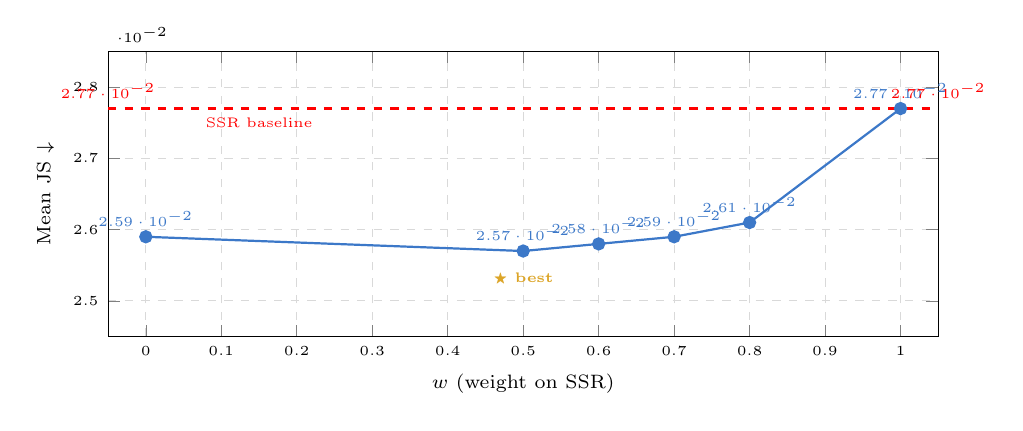
\begin{tikzpicture}
\begin{axis}[
  width=\linewidth, height=5.2cm,
  xlabel={$w$ (weight on SSR)}, ylabel={Mean JS $\downarrow$},
  xlabel style={font=\scriptsize}, ylabel style={font=\scriptsize},
  xticklabel style={font=\tiny}, yticklabel style={font=\tiny},
  ymin=0.0245, ymax=0.0285, xmin=-0.05, xmax=1.05,
  grid=both, grid style={dashed, gray!30},
  mark options={solid, fill=barblue},
  nodes near coords, nodes near coords style={font=\tiny},
  every axis plot/.append style={thick},
]
\addplot[color=barblue, mark=*] coordinates {
  (0.0, 0.0259) (0.5, 0.0257) (0.6, 0.0258)
  (0.7, 0.0259) (0.8, 0.0261) (1.0, 0.0277)};
\addplot[color=red, dashed, mark=none] coordinates {(-0.05, 0.0277) (1.05, 0.0277)};
\node[red, font=\tiny] at (axis cs:0.15, 0.0275) {SSR baseline};
\node[bargold, font=\tiny\bfseries] at (axis cs:0.5, 0.0253) {$\bigstar$ best};
\end{axis}
\end{tikzpicture}
\\[2pt]
{\footnotesize LLM-dist alone ($w{=}0$) nearly matches the best mix; SSR contributes a small correction at $w{=}0.5$.}
\end{minipage}
\hfill
\begin{minipage}[t]{0.48\textwidth}
\section*{5. M4 weight sweep (SSR + ML-steer)}
\centering
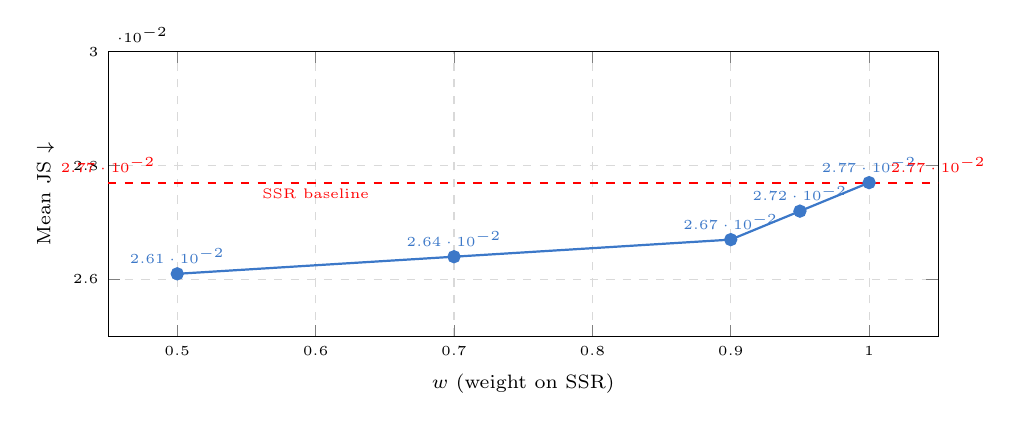
\begin{tikzpicture}
\begin{axis}[
  width=\linewidth, height=5.2cm,
  xlabel={$w$ (weight on SSR)}, ylabel={Mean JS $\downarrow$},
  xlabel style={font=\scriptsize}, ylabel style={font=\scriptsize},
  xticklabel style={font=\tiny}, yticklabel style={font=\tiny},
  ymin=0.025, ymax=0.030, xmin=0.45, xmax=1.05,
  grid=both, grid style={dashed, gray!30},
  mark options={solid, fill=barblue},
  nodes near coords, nodes near coords style={font=\tiny},
  every axis plot/.append style={thick},
]
\addplot[color=barblue, mark=*] coordinates {
  (0.5, 0.0261) (0.7, 0.0264) (0.9, 0.0267) (0.95, 0.0272) (1.0, 0.0277)};
\addplot[color=red, dashed, mark=none] coordinates {(0.45, 0.0277) (1.05, 0.0277)};
\node[red, font=\tiny] at (axis cs:0.60, 0.0275) {SSR baseline};
\end{axis}
\end{tikzpicture}
\\[2pt]
{\footnotesize Steering helps only as a minority voice; $w{=}0.5$ gives the largest independent gain.}
\end{minipage}

\vspace{10pt}

\begin{minipage}[t]{0.48\textwidth}
\section*{6. Multi-layer steering alone (M3)}
\centering\small
\begin{tabular}{@{}lc@{}}
\toprule
Layer set $L$ & Mean JS \\
\midrule
$[16, 24]$              & 0.0378 \\
$[20, 24]$              & 0.0404 \\
$[16, 20, 24, 28]$      & 0.0434 \\
$[12, 16, 20, 24]$      & 0.0643 \\
\rowcolor{badrow} Single L24, $\alpha$=0.1 & 0.0659 \\
\bottomrule
\end{tabular}
\\[2pt]
{\footnotesize M3 alone never beats M0; it is useful only via the M4 ensemble.}
\end{minipage}
\hfill
\begin{minipage}[t]{0.48\textwidth}
\section*{7. M5 SSR knob tuning}
\centering\small
\begin{tabular}{@{}llc@{}}
\toprule
Axis & Setting & Mean JS \\
\midrule
\multirow{3}{*}{Posts/cluster $n$} & 30 & 0.0277 \\
 & 50 & 0.0275 \\
 & 80 & 0.0276 \\
\midrule
\multirow{4}{*}{Top-$K$ clusters} & 5  & 0.0272 \\
 & 10 & 0.0272 \\
 & 15 & 0.0277 \\
 & 20 & 0.0280 \\
\bottomrule
\end{tabular}
\\[2pt]
{\footnotesize Effects within noise; tuning SSR alone cannot replace the ensemble.}
\end{minipage}

\vspace{10pt}

\section*{8. Negative results (methods that do NOT beat pure SSR)}

\centering\small
\begin{tabular}{@{}lcc@{}}
\toprule
Method & Mean JS & vs M0 \\
\midrule
\rowcolor{badrow} Per-post LLM voting (ask LLM per post)        & 0.2360 & +755\% \\
\rowcolor{badrow} Large $\alpha{=}1.0$ steering, unit-normed    & 0.0689 & +149\% \\
\rowcolor{badrow} Single-layer steer L24, $\alpha{=}0.1$        & 0.0659 & +138\% \\
\rowcolor{badrow} Persona-projected SSR, $s$=0.1                & 0.0560 & +102\% \\
\rowcolor{badrow} Persona-projected SSR, $s$=0.3                & 0.0478 & +73\% \\
Persona-projected SSR, $s$=0.5                                  & 0.0405 & +46\% \\
ICL with 5 example posts                                        & 0.0368 & +33\% \\
SSR + per-post LLM correction (not dist estimation)             & 0.0296 & +7\% \\
\midrule
SSR + KL-penalty demographic reweight (from 23Q run)$^\dagger$  & $\approx$baseline & --- \\
SSR + KL + QAW (from 23Q run)$^\dagger$                         & $\approx$baseline & --- \\
\bottomrule
\end{tabular}
\\[2pt]
{\footnotesize $^\dagger$ Earlier 23Q-set claims; 23Q questions are LLM-generated synthetic items and do not reflect real reconstruction performance. Quarantined.}
\flushleft

\vspace{8pt}\hrule\vspace{4pt}

\textbf{TL;DR.}
(1) \textbf{SSR + LLM-dist at $w{=}0.5$} is the lead method: Mean JS $=$ \textbf{0.0257}, a \textbf{7.2\%} reduction over pure SSR.
(2) The \textbf{LLM-dist} component carries most of the gain; SSR adds a small correction at 50/50 mix.
(3) A second, \textbf{independent} contributor is the \textbf{SSR + multi-layer-steering ensemble} (M4), $-$5.4\% at $w{=}0.5$; combining M2 + M4 is untested.
(4) All single-layer steering, per-post LLM voting, persona-projection, and demographic KL/QAW methods are neutral or harmful.

\vspace{4pt}
{\footnotesize \textit{Sources:} \texttt{results/improve\_orig6.json} (2026-04-21), \texttt{results/persona\_methods.json} (2026-04-20), \texttt{results/fix\_steering\_results.json} (2026-04-19).}

\end{document}
